\documentclass[11pt,a4paper,english]{article}
\usepackage{babel}
\usepackage{amsmath,amssymb,amsfonts}
\usepackage{graphicx,subfigure,epsfig}
\usepackage[export]{adjustbox}    % for positioning figure
\usepackage{textcomp}
\usepackage[usenames,dvipsnames,svgnames,table]{xcolor}

% for listing
\usepackage{enumitem}
\usepackage[ampersand]{easylist}
\ListProperties(Hide=100, Hang=true, Progressive=3ex, Style*=-- ,
Style2*=$\bullet$ ,Style3*=$\circ$ ,Style4*=\tiny$\blacksquare$ )    % for easylist

% for hyperlink
\usepackage{url}
\usepackage{hyperref}
\hypersetup{colorlinks=true,linkcolor=blue,filecolor=magenta,urlcolor=cyan}

% from lalit
%\usepackage{bm}
%\usepackage{latexsym}
%\usepackage{dcolumn}
%\usepackage{psfrag}
%\usepackage{gensymb}
%\usepackage{placeins}
%
%\usepackage[stable]{footmisc}

% Creating Title for the assesment

\title{Assignment 2}
\author{Bhishan Poudel}
\date{Sep, 2015}
% Don't forget to use \maketitle below \begin{document}

\begin{document}
\maketitle
\tableofcontents
\listoffigures
\clearpage

\section{Care in evaluating functions}

	%%%%% including figure %%%%%%%%%%%%%%%%%%
	\begin{figure}
	\centering
	
\includegraphics[width=1.0\textwidth,left]{./images/a.jpg}
	\caption{Plot of x vs $x - sin(x)$ }
	\end{figure}
	
	
	\begin{figure}
	
	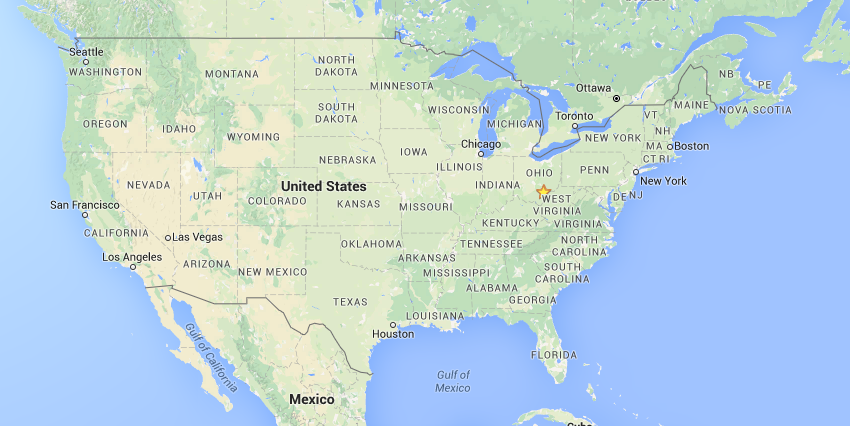
\includegraphics[width=1.0\textwidth,left]{./images/usa_map.png}
	\caption{Usa map }
	\end{figure}
	%%%%%%%%%%%%%%%%%%%%%%%%%%%%%%%%%%%%%%%%%%
\end{document}

